\section{Проектирование персонального ассистента организации времени обучающихся}
\label{sec:designing}

Целью данного раздела является преобразование теоретических выводов и выявленных проблем в конкретные проектные решения. В рамках раздела будут определены концептуальные и технические требования к разрабатываемой системе, спроектирована логическая архитектура взаимодействия компонентов, а также разработана модель данных. Итогом раздела выступит полная спецификация, служащая базисом для программной реализации интеллектуального ассистента.

\subsection{Концептуальные границы и требования к системе}

Основополагающей бизнес-целью разрабатываемого программного решения является компенсация когнитивных факторов академической прокрастинации путем делегирования рутинных процессов планирования интеллектуальному агенту.

Как итог аналитического раздела, были сформулированы функциональные требования к ассистенту, которые отражают пути достижения цели проекта, через реализацию определённого функционала. Как отмечалось, ассистент должен выполнять задачи организационного характера. Но для того, чтобы чётко определить границы функционала и возможности ассистента, следует привести варианты использования для различных пользователей системы. 

Исходя из ограничений предметной области, будем анализировать сегмент обучающихся пользователей и рассмотрим их роли в системе.

\subsubsection{Ключевые пользователи системы}

Целевой аудиторией продукта являются обучающиеся высших учебных заведений, а также лица, занимающиеся самообразованием и проектной деятельностью. Поскольку система позиционируется как персональный ассистент, архитектура взаимодействия подразумевает наличие единственной системной роли - Пользователь.
Функциональные границы проекта определены следующими базовыми прецедентами взаимодействия пользователя с системой, представленными на диаграмме \ref{fig:use-case}:
\begin{figure}[H]
\centering
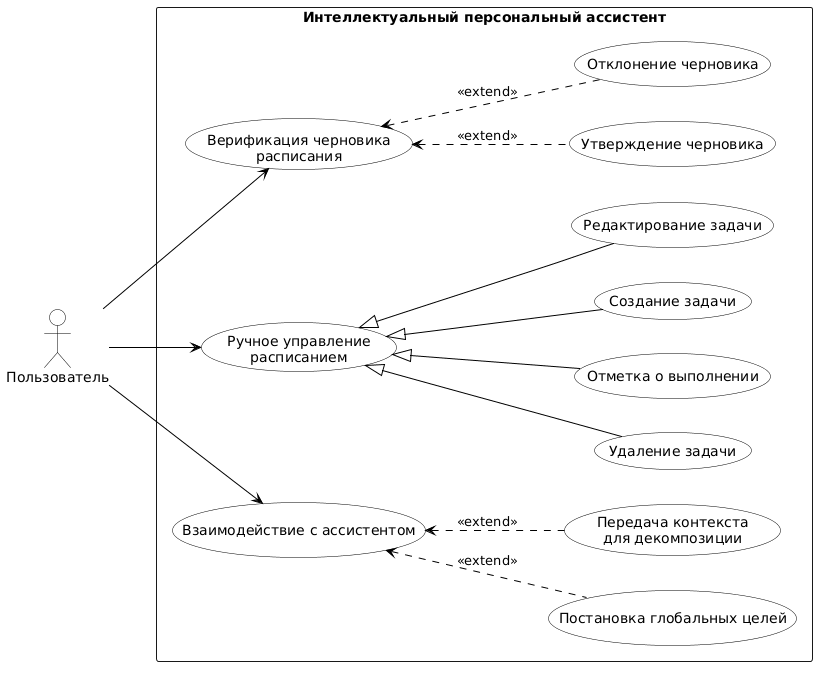
\includegraphics[width=0.85\linewidth]{picture/diagrams/use-case.png}
\caption{Диаграмма вариантов использования системы}
\label{fig:use-case}
\end{figure}

Специфика ориентации на обучающихся должна выражаться в доменной адаптации алгоритмов: в запросах к языковой модели используют промпты (Prompts) с учетом академического контекста (типовых структур курсовых и лабораторных работ), а архитектура данных должна учитывать цикличность учебного процесса (семестры, сессии, дедлайны по дисциплинам). Пример системного промпта представлен в приложении А. %\ref{appendix:prompt}.



\subsubsection{Нефункциональные требования и ограничения}

Проектирование системы ведется с учетом ресурсных ограничений, характерных для этапа разработки минимально жизнеспособного продукта (MVP): фиксированного бюджета, сжатых сроков разработки и малого размера команды. В связи с этим задачи обеспечения промышленного горизонтального масштабирования и сверхвысокой доступности на данном этапе исключены из фокуса. 

Тем не менее, архитектурные решения принимаются с заделом на будущее развитие системы и соблюдение нормативных норм. Основной упор делается на следующие нефункциональные требования:

\begin{enumerate}[label=\arabic*]
    
    \item Безопасность и защита персональных данных. В соответствии с законодательством о персональных данных (в частности, Законом РБ «О защите персональных данных»), система должна обеспечивать конфиденциальность пользовательской информации. Архитектура должна предусматривать возможность безопасной реализации внешней аутентификации, в том числе через протокол OAuth 2.0, исключающий передачу паролей сторонним сервисам.
    
    \item Изолированность состояния и верифицируемость. Для минимизации рисков, связанных с галлюцинациями языковых моделей, должен быть реализован принцип подтвержденного действия: любые изменения в базе данных расписания возможны только после явной валидации сформированного системой промежуточного результата пользователем.
    
    \item Принципы расширяемой архитектуры. Код и структура базы данных проектируются согласно принципам SOLID и модульности. Это необходимо для обеспечения низкой стоимости поддержки и возможности быстрого добавления новых модулей без полной переработки ядра системы.
\end{enumerate}



\subsubsection{Логическая архитектура и технические требования} 

Для обеспечения заявленного функционала система должна быть спроектирована на основе модульной логической архитектуры, разделяющей зоны ответственности между интерфейсом, маршрутизацией запросов и когнитивной обработкой данных.
Логический поток обработки пользовательского запроса представлен на диаграммах \ref{fig:sequence-gen-p1}, \ref{fig:sequence-gen-p2} и \ref{fig:sequence-draft}, и затрагивает следующие модули:

\begin{enumerate}[label=\arabic*]
    \item Гибридный интерфейс, совмещающий чат и календарную сетку. Должен уметь отправлять намерения пользователя на сервер и асинхронно отрисовывать полученные «черновики» расписания в виде графических карточек для последующей верификации. 
    \item Серверный маршрутизатор, отвечающий за прием запросов, авторизацию пользователя и управление сессиями. Выступает оркестратором. Получая текстовый запрос, бэкенд обогащает его системным контекстом (текущее время, занятые слоты из хранилища) и передает в Агентный модуль.
    \item Агентный модуль, предназначенный для семантического анализа естественного языка, декомпозиции задач и поиска оптимальных временных слотов. Стоит отметить, что поиск оптимальных слотов осуществляется алгоритмически.
    \item Модуль не имеет прямого доступа к модификации базы данных. Результатом его работы является строго структурированный транзакционный объект (Draft), описывающий предлагаемые изменения в расписании.
    \item Система хранения данных. Её назначение - персистентное хранение информации о пользователях, их задачах и токенах авторизации. Использование реляционной модели данных для обеспечения строгих связей между задачами, подзадачами и временными интервалами.
\end{enumerate}

\begin{figure}[H]
\centering
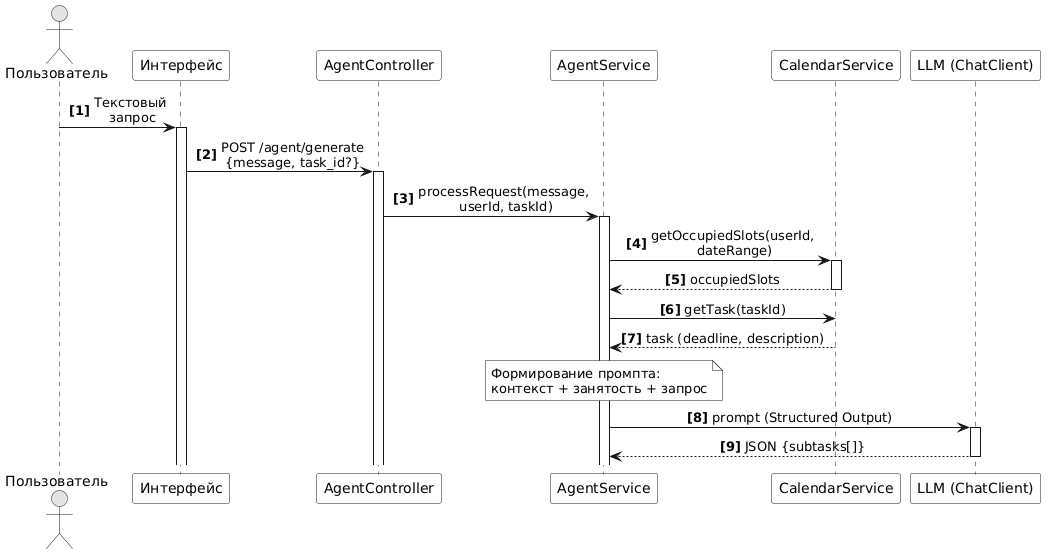
\includegraphics[width=1.0\linewidth]{picture/diagrams/sequence_generation_p1.png}
\caption{Диаграмма последовательности генерации расписания: сбор контекста и вызов языковой модели}
\label{fig:sequence-gen-p1}
\end{figure}

\begin{figure}[H]
\centering
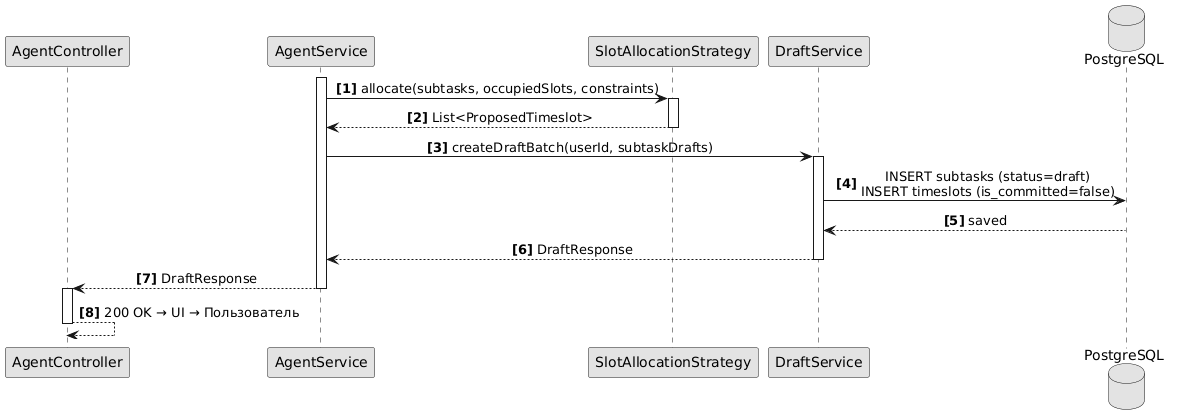
\includegraphics[width=1.0\linewidth]{picture/diagrams/sequence_generation_p2.png}
\caption{Диаграмма последовательности генерации расписания: алгоритм размещения и сохранение черновика}
\label{fig:sequence-gen-p2}
\end{figure}

\begin{figure}[H]
\centering
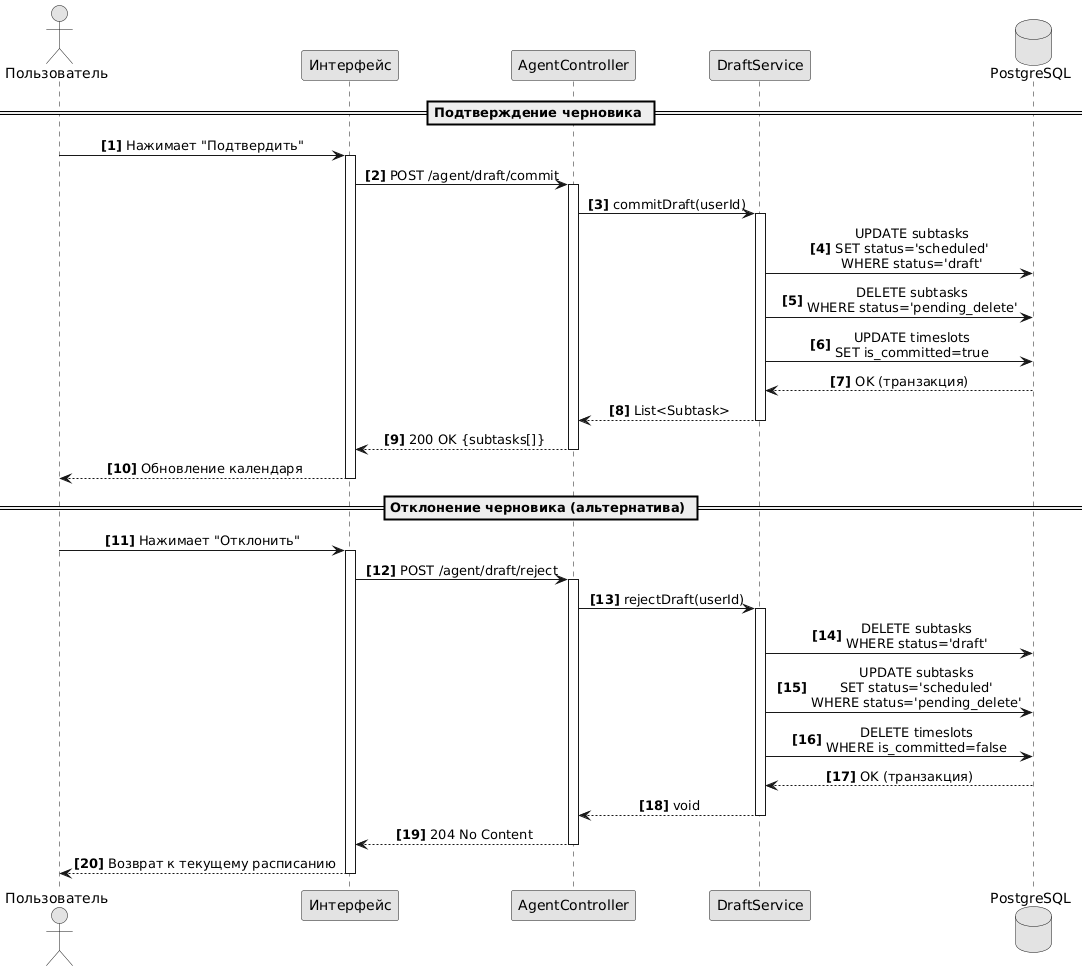
\includegraphics[width=1.0\linewidth]{picture/diagrams/sequence_draft.png}
\caption{Диаграмма последовательности подтверждения и отклонения черновика}
\label{fig:sequence-draft}
\end{figure}


Разделение системы на описанные модули позволяет изолировать стохастическую природу языковых моделей от жесткой транзакционной логики сохранения данных, обеспечивая надежность и расширяемость программного комплекса.

\subsection{Архитектура системы}

Принимая во внимание требования к изоляции когнитивного агента от бизнес-транзакций, в качестве глобального архитектурного паттерна выбрана многоуровневая архитектура в формате модульного монолита. Данный подход обеспечивает оптимальный баланс между скоростью разработки продукта и возможностью его дальнейшего горизонтального масштабирования или разделения на микросервисы. 

Поскольку целевая аудитория взаимодействует с объемными академическими материалами и нуждается в наглядной визуализации расписания, целевой платформой определено Web-приложение. Взаимодействие между клиентской частью и сервером реализуется по архитектурному стилю REST (Representational State Transfer) поверх протокола HTTP. Логически серверная часть приложения разделена на независимые слои (данных, бизнес-логики и контроллеров), взаимодействующие друг с другом посредством строгих интерфейсов.

\subsubsection{Модель данных}

В основе проектирования системы лежит предметно-ориентированный подход. Глобальная модель данных носит гибридный характер:
\begin{enumerate}[label=\arabic*]
    \item Реляционная модель (рисунок \ref{fig:er}) отвечает за строгую транзакционную целостность. Ключевыми бизнес-сущностями выступают: пользователь, способ входа, учебная задача, подзадача и временной слот. Реляционная структура гарантирует невозможность коллизий на уровне ограничений базы данных.
    \item Векторная модель — вспомогательная подсистема для реализации долгосрочной памяти ассистента. Предназначена для хранения эмбеддингов методических указаний, учебных планов и истории взаимодействия, что позволяет языковой модели извлекать семантический контекст при декомпозиции новых задач.
\end{enumerate}

\begin{figure}[H]
\centering
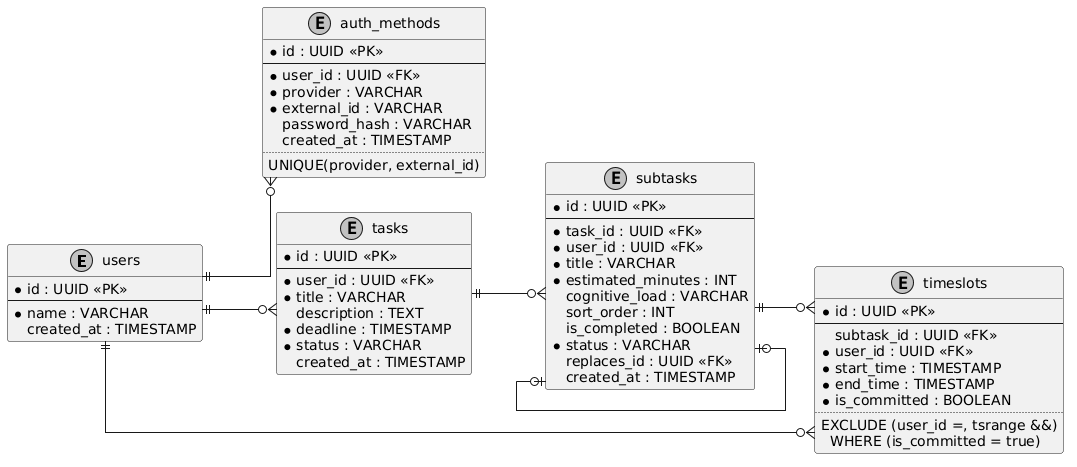
\includegraphics[width=0.9\linewidth]{picture/diagrams/er.png}
\caption{Диаграмма отношения сущностей}
\label{fig:er}
\end{figure}

Разработанная диаграмма отражает нормализованную структуру реляционной базы данных. Физическая невозможность временных коллизий гарантируется на уровне СУБД за счёт следующих механизмов:
\begin{enumerate}[label=\arabic*]
    \item Изоляция состояний реализована через статусную модель подзадач. Черновые подзадачи со статусом «draft» не влияют на основное расписание и становятся активными только после явного подтверждения пользователем в рамках одной транзакции.
    \item Для таблицы временных слотов задано ограничение исключения, запрещающее сохранение пересекающихся диапазонов для подтверждённых слотов одного пользователя. База данных физически отклонит транзакцию с накладывающимся временем.
    \item Порядок выполнения подзадач задаётся целочисленным полем сортировки, а рекурсивная связь замены позволяет агенту предлагать модификации существующих подзадач без их немедленного удаления.
\end{enumerate}

\subsubsection{Слой данных}

Слой данных изолирует инфраструктурную логику работы с хранилищами от остального приложения. Он реализуется с использованием паттерна «Репозиторий». Данный слой инкапсулирует SQL-запросы к реляционной СУБД и вызовы к векторному хранилищу. Благодаря такому уровню абстракции, бизнес-логика оперирует исключительно объектами-сущностями, оставаясь независимой от конкретных реализаций баз данных.

Каждая бизнес-сущность из модели данных отображается в классы-сущности средствами объектно-реляционного отображения. Репозитории представляют собой интерфейсы, определяющие контракт доступа к данным без привязки к конкретным SQL-запросам.

На рисунке \ref{fig:repo-user-auth} представлены репозитории для работы с пользователями и способами аутентификации. Они обеспечивают базовые операции поиска, сохранения и удаления соответствующих сущностей.

\begin{figure}[H]
\centering
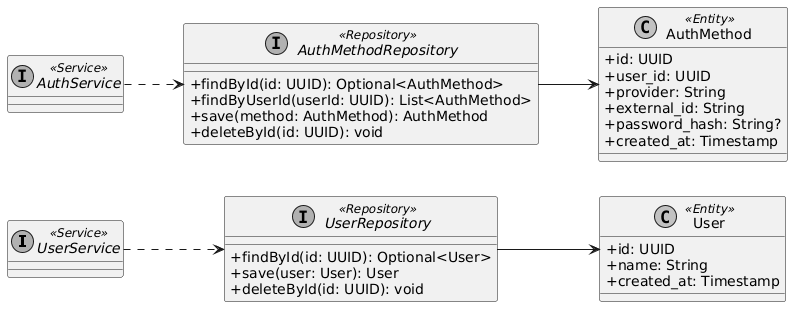
\includegraphics[width=0.85\linewidth]{picture/diagrams/class_repository_user_auth.png}
\caption{Диаграмма классов слоя данных: пользователи и аутентификация}
\label{fig:repo-user-auth}
\end{figure}

На рисунке \ref{fig:repo-calendar} представлены репозитории календарного домена. Репозиторий задач предоставляет фильтрацию по пользователю. Репозиторий подзадач поддерживает выборку с сортировкой и фильтрацию по статусу. Репозиторий временных слотов обеспечивает выборку по диапазону дат и признаку подтверждения.

\begin{figure}[H]
\centering
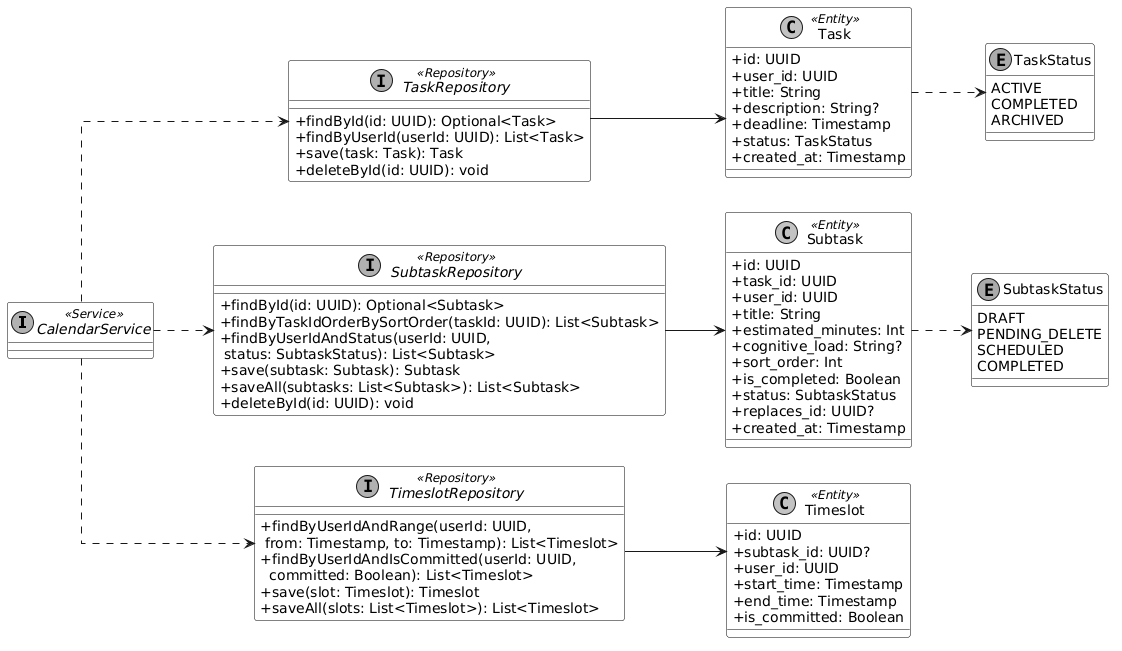
\includegraphics[width=1.0\linewidth]{picture/diagrams/class_repository_calendar.png}
\caption{Диаграмма классов слоя данных: календарный домен}
\label{fig:repo-calendar}
\end{figure}

На рисунке \ref{fig:repo-agent} представлены репозитории, используемые агентным модулем для работы с черновиками. Здесь же показан интерфейс векторного хранилища, обеспечивающий семантический поиск по сохранённым документам для обогащения контекста при обращении к языковой модели.

\begin{figure}[H]
\centering
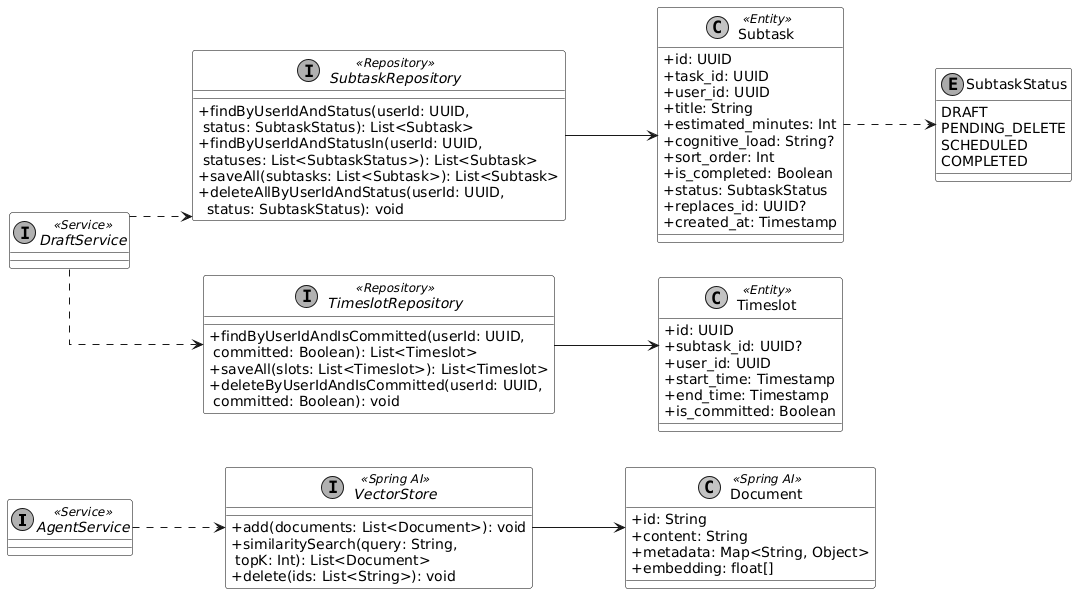
\includegraphics[width=1.0\linewidth]{picture/diagrams/class_repository_agent.png}
\caption{Диаграмма классов слоя данных: агентный модуль и векторное хранилище}
\label{fig:repo-agent}
\end{figure}

\subsubsection{Слой бизнес-логики}

Слой бизнес-логики (сервисный слой) является центральным ядром системы, агрегирующим вызовы к репозиториям и внешним компонентам. Именно здесь реализуется ключевая ценность интеллектуального ассистента. В его ответственность входит:
\begin{itemize}
    \item оркестрация взаимодействия с внешними языковыми моделями;
    \item управление жизненным циклом черновика расписания для реализации паттерна подтверждённого действия (генерация, ожидание верификации, подтверждение или откат);
    \item выполнение детерминированных алгоритмов размещения подзадач во временные слоты;
    \item обеспечение транзакционности операций.
\end{itemize}

Сервисный слой разделён на три функциональные группы. На рисунке \ref{fig:service-user-auth} представлены сервисы пользователей и аутентификации, отвечающие за базовые операции управления учётными записями и способами входа.

\begin{figure}[H]
\centering
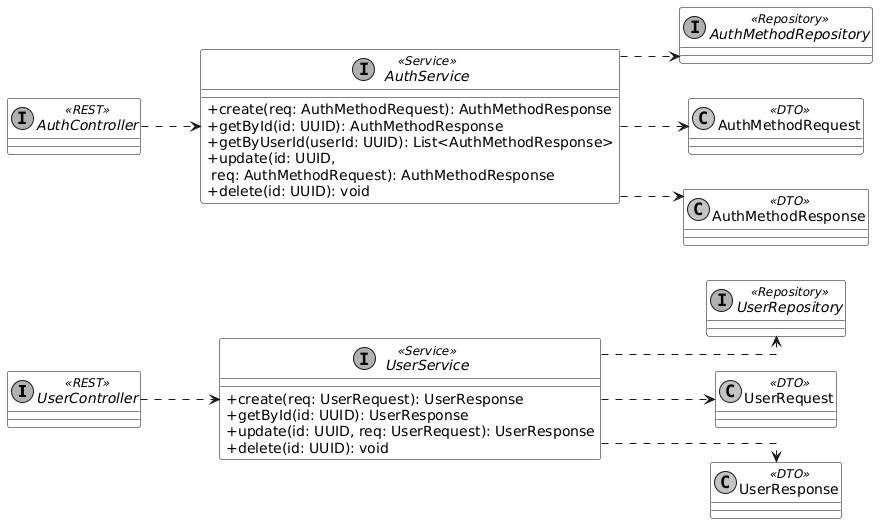
\includegraphics[width=0.85\linewidth]{picture/diagrams/class_service_user_auth.png}
\caption{Диаграмма классов сервисного слоя: пользователи и аутентификация}
\label{fig:service-user-auth}
\end{figure}

На рисунке \ref{fig:service-calendar} представлен календарный сервис, объединяющий операции над задачами, подзадачами и временными слотами в единый транзакционный контекст. Объединение обусловлено сильной связностью домена: создание подзадачи и её временного слота должно выполняться атомарно.

\begin{figure}[H]
\centering
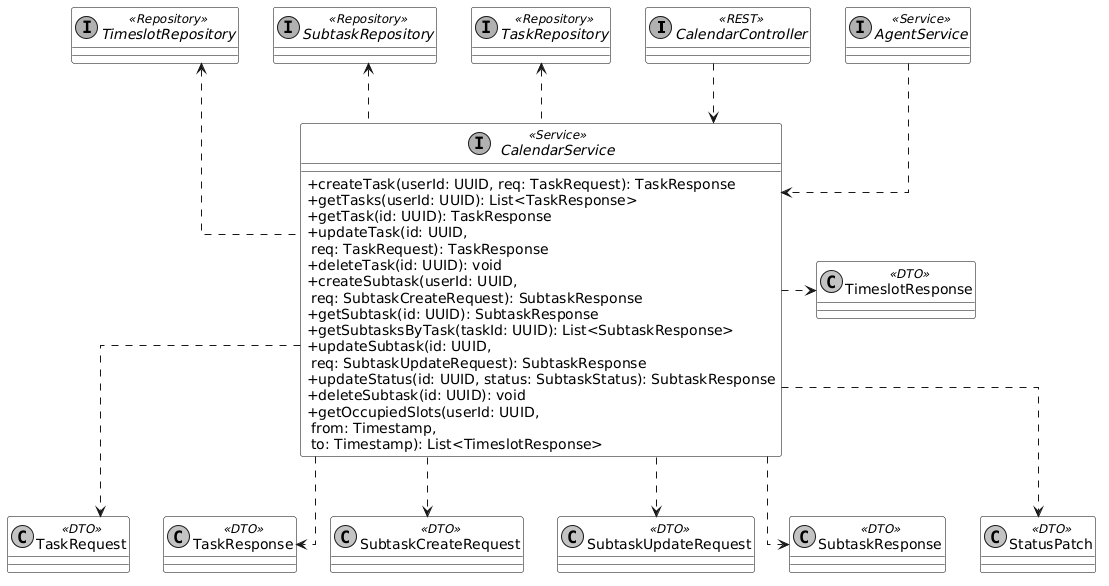
\includegraphics[width=1.0\linewidth]{picture/diagrams/class_service_calendar.png}
\caption{Диаграмма классов сервисного слоя: календарный домен}
\label{fig:service-calendar}
\end{figure}

На рисунке \ref{fig:service-agent} представлены сервисы агентного модуля. Сервис агента выступает оркестратором: принимает запрос пользователя, собирает контекст через календарный сервис, выполняет семантический поиск в векторном хранилище, формирует обогащённый запрос к языковой модели, а полученный результат передаёт алгоритму размещения слотов. Сервис черновиков управляет жизненным циклом предложенных изменений — от создания до подтверждения или отклонения.

\begin{figure}[H]
\centering
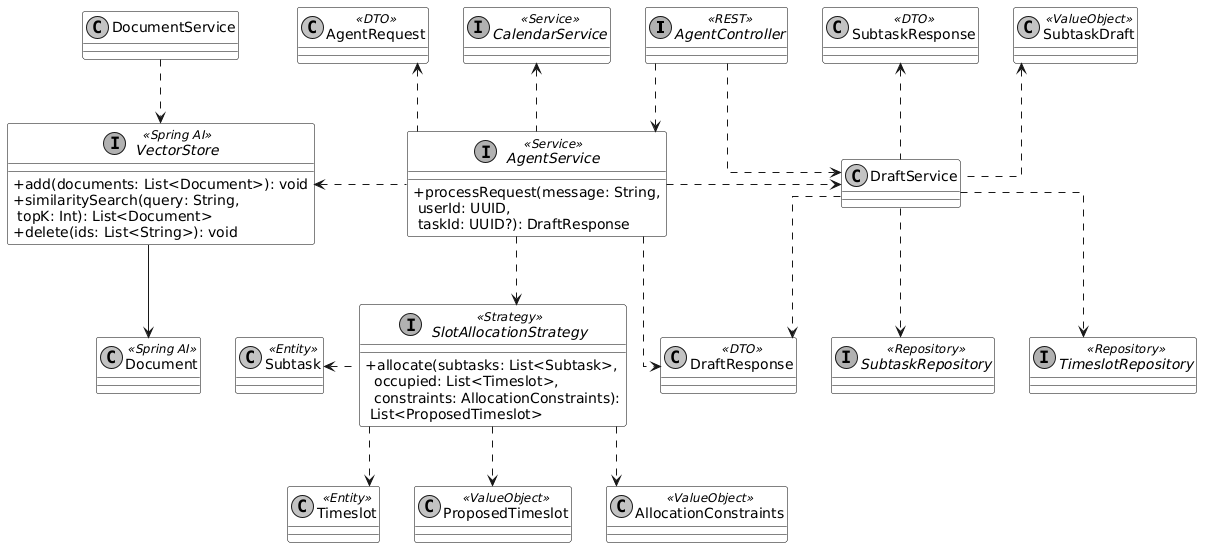
\includegraphics[width=1.0\linewidth]{picture/diagrams/class_service_agent.png}
\caption{Диаграмма классов сервисного слоя: агентный модуль и управление черновиками}
\label{fig:service-agent}
\end{figure}

Слабая связность сервисного слоя обеспечивает высокую тестируемость алгоритмов планирования без необходимости поднятия реальной базы данных или сетевого окружения.

\subsubsection{Слой контроллеров}

Слой контроллеров выступает в роли единого шлюза для приёма внешних запросов от клиентского приложения. Он реализует набор маршрутов в стиле REST. Основная задача данного слоя — маршрутизация запросов, десериализация входящих данных в объекты передачи данных, первичная валидация полей и передача управления слою бизнес-логики. На этом же уровне реализуется проверка токенов авторизации для контроля сессий.

На рисунке \ref{fig:ctrl-user-auth} представлены контроллеры управления пользователями и способами аутентификации с соответствующими объектами передачи данных.

\begin{figure}[H]
\centering
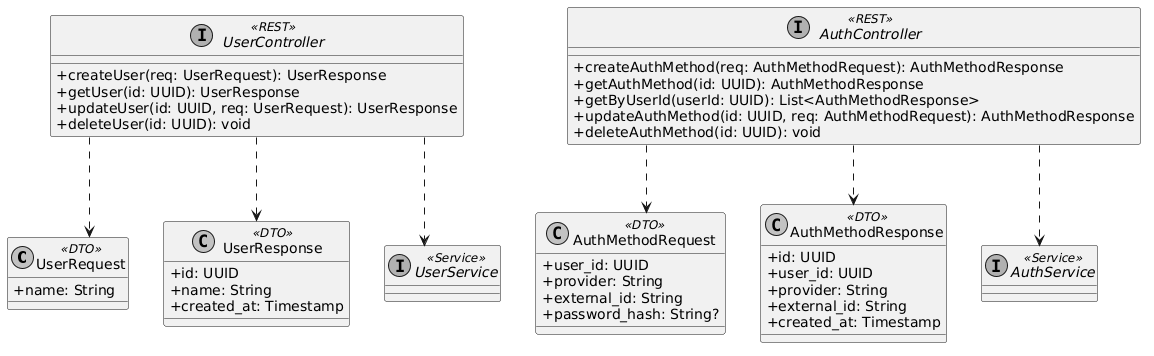
\includegraphics[width=0.85\linewidth]{picture/diagrams/controller_user_auth.png}
\caption{Диаграмма классов слоя контроллеров: пользователи и аутентификация}
\label{fig:ctrl-user-auth}
\end{figure}

На рисунке \ref{fig:ctrl-calendar} представлен контроллер календарного домена, обеспечивающий операции над задачами, подзадачами и временными слотами.

\begin{figure}[H]
\centering
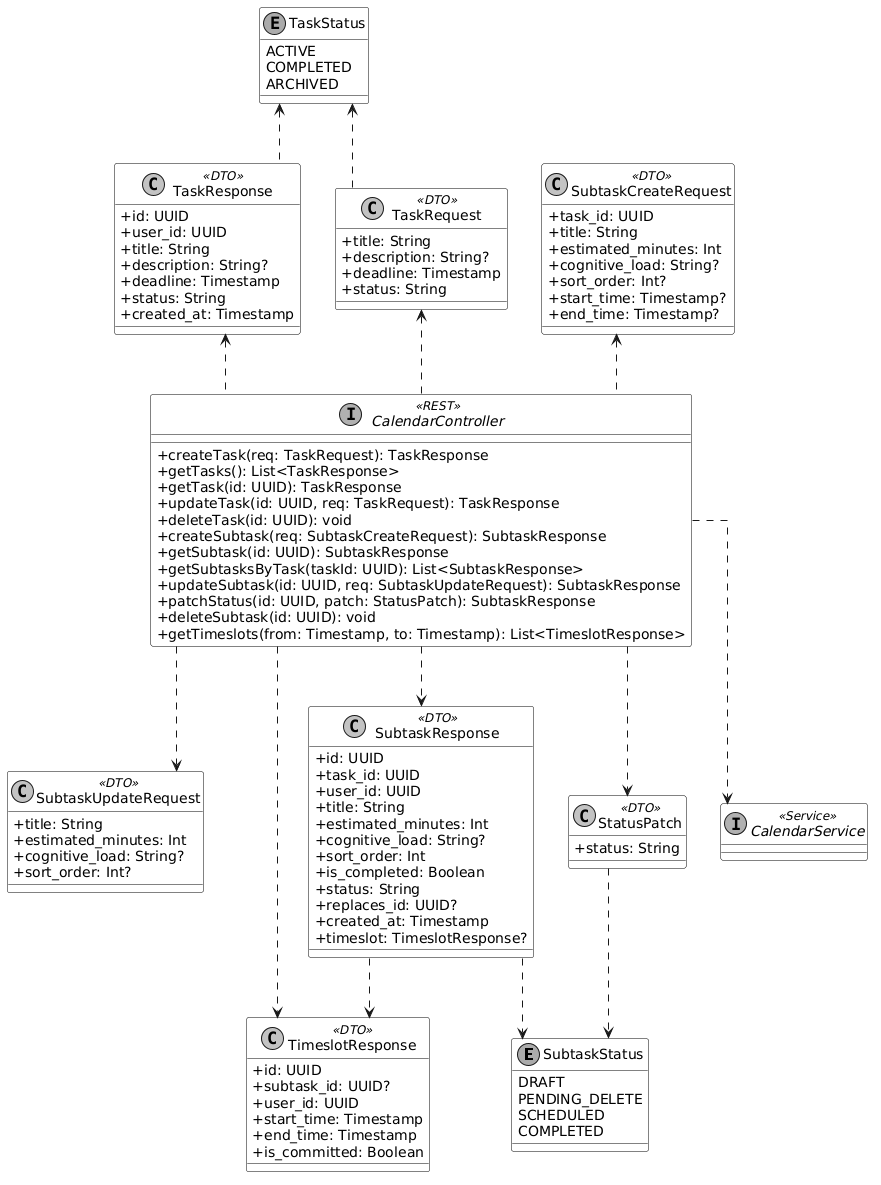
\includegraphics[width=1.0\linewidth]{picture/diagrams/contoller_calendar.png}
\caption{Диаграмма классов слоя контроллеров: календарный домен}
\label{fig:ctrl-calendar}
\end{figure}

На рисунке \ref{fig:ctrl-agent} представлен контроллер агентного модуля, принимающий запросы на генерацию расписания и управление черновиком.

\begin{figure}[H]
\centering
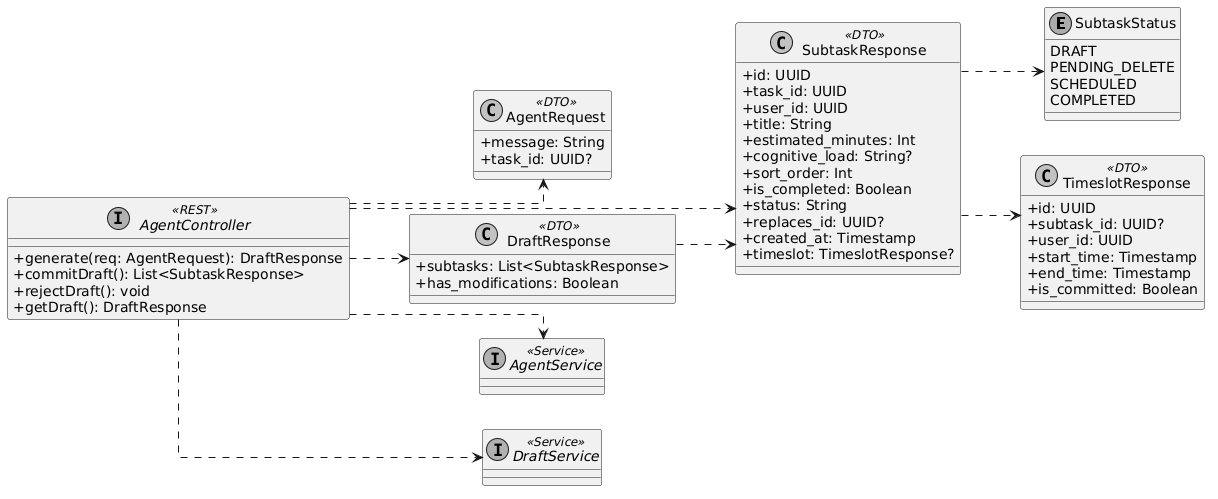
\includegraphics[width=0.85\linewidth]{picture/diagrams/controller_agent.png}
\caption{Диаграмма классов слоя контроллеров: агентный модуль}
\label{fig:ctrl-agent}
\end{figure}

Контроллеры не имеют прямого доступа к репозиториям или базе данных, а взаимодействуют с ними строго через сервисный слой, что подтверждается зависимостями на приведённых диаграммах.

\subsubsection{Пользовательский интерфейс}

Для обеспечения интерактивности пользовательский интерфейс проектируется как одностраничное Web-приложение. Классические решения, такие как прямая интеграция ИИ в Google Calendar, признаны нецелесообразными в рамках текущих требований, так как сторонние интерфейсы не позволяют реализовать гибридный агентный пользовательский интерфейс.

Разрабатываемый интерфейс должен визуально разделяться на две функциональные зоны: диалоговое окно для текстового взаимодействия с агентом и динамическую календарную сетку, как на схеме \ref{fig:ui}. Сгенерированные агентом «черновики» расписания должны рендериться непосредственно в диалоговом окне в виде интерактивных виджетов с возможностью их утверждения или отклонения. Визуальная статистика прогресса выполнения задач формируется клиентской частью на основе данных, уже получаемых через существующие эндпоинты календарного домена, и не требует выделенного серверного модуля.

\begin{figure}[H]
\centering
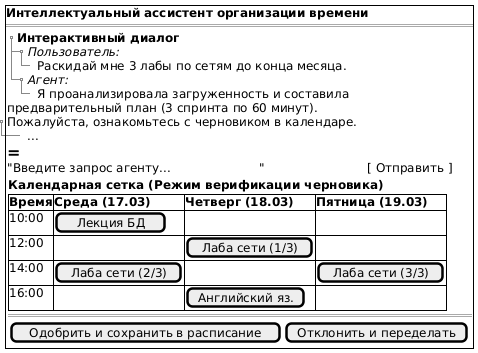
\includegraphics[width=1.0\linewidth]{picture/ui.png}
\caption{Диаграмма интерфейса системы}
\label{fig:ui}
\end{figure}

\subsection{Вывод}

В рамках данного раздела был выполнен комплексный этап логического и архитектурного проектирования системы интеллектуального персонального ассистента, направленный на трансляцию теоретических концепций в строгие технические спецификации. 

В ходе работы были определены границы проекта и сформированы концептуальные требования для целевой аудитории. Спроектированная диаграмма прецедентов позволила формализовать базовые сценарии взаимодействия пользователя с системой, ключевым из которых является верификация предложенных расписаний.

Для обеспечения надежности и масштабируемости программного комплекса была спроектирована многоуровневая архитектура по шаблону модульного монолита. Разработанная диаграмма последовательности наглядно продемонстрировала механизмы изоляции когнитивного ядра от бизнес-транзакций, подтвердив жизнеспособность выбранного нейросимволического подхода и паттерна Human-in-the-Loop. 

Особое внимание было уделено проектированию слоя хранения данных. Сформированная ER-диаграмма описывает нормализованную реляционную модель, которая на уровне ограничений базы данных гарантирует защиту от временных коллизий и галлюцинаций планирования. Кроме того, заложен гибридный векторно-реляционный подход для реализации долгосрочной памяти ассистента (RAG).

Таким образом, в результате проектирования сформирован исчерпывающий пакет архитектурных, алгоритмических и схемотехнических решений. Спроектированные модели взаимодействия компонентов, доменная структура данных и спецификации гибридного пользовательского интерфейса  полностью отвечают поставленным целям и служат надежным инженерным фундаментом для перехода к следующему этапу исследования — непосредственной программной реализации разрабатываемого продукта.

